\section{Anwendungen und Beispiele}

\subsection{Charakteristika eines Geigentons}
Die naheliegendste Anwendung ist die Analyse des Schwingungsverhaltens von Musikinstrumenten, in unserem Falle einer Geige. Wenn der Bogen über die Saiten gezogen wird entsteht eine angeregt Schwingung auf der Saite. Der Steg am unteren Ende des Instrument und der Finger auf dem Griffbrett bilden zwei feste Enden, sodass sich eine stehende Welle auf der Saite ausbilden muss. Die Saitenlänge muss dabei ein Vielfaches der Wellenlänge sein.
\begin{align}
  l = \frac{k}{2} \lambda && k \in \mathbb{N}
\end{align}

In Abbildung \ref{img:violin} ist das Spektrogramm einer Geige gezeigt. Die roten Frequenzstreifen entsprechen den erwarteten Grund- und Oberschwingungen. Da die Saite ständig von au\ss en angeregt wird entsteht ein Dauerton. Fällt diese Anregung weg, wie im Bereich ab $t_1 = 1,25sec.$, dann klingt der Ton der Saite aus. Charakteristisch ist dabei vor allem, dass die Obertöne zuerst verschwinden.

Wird beim Spielen des Tons nicht die Spielweise des Vibrato verwendet, können sich nur stehende Wellen mit wenigen Oberschwingungen ausbilden. Der Ton klingt dann scharf und unharmonisch.

\begin{figure*}
  \centering
  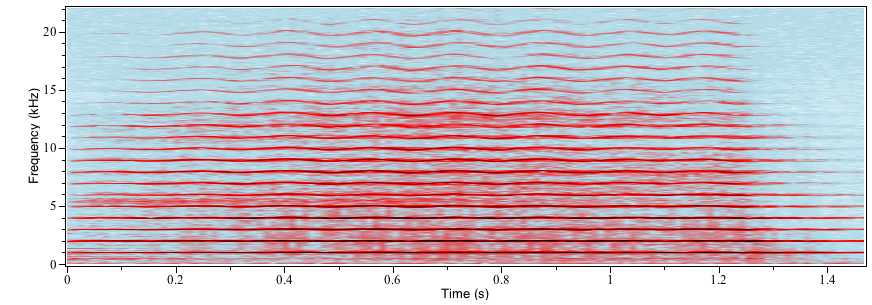
\includegraphics[width=\linewidth]{img/violin}
  \caption{Spektrogramm eines Geigentons mit Vibrato. Quelle: (\url{ http://www.maplesoft.com/products/maple/features/Signal_Processing.aspx},  21.11.15)}
  \label{img:violin}
\end{figure*}
\begin{figure*}
  \centering
  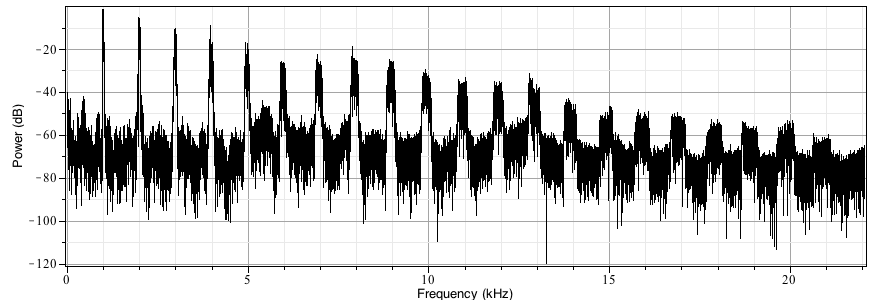
\includegraphics[width=\linewidth]{img/violin_power}
  \caption{Frequenzspektrum eines Geigentons mit Vibrato. Quelle: (\url{ http://www.maplesoft.com/products/maple/features/Signal_Processing.aspx},  21.11.15)}
  \label{img:violin_power}
\end{figure*}

\subsection{Quantenmechanik}
Jeder Zustand der klassichen Mechanik kann durch Position und Impuls $ \langle \vec{x}, \vec{p} \rangle $ eindeutig beschrieben werden.
In der Quantenmechanik sind jedoch Position und Impuls unscharfe Grö\ss en. Daher wird ein Zustand durch die komplexe Wellenfunktion $ \Psi(x,t) $ beschrieben.

Um nun Informationen über den Zustand zu erhalten, werden lineare Differenzialoperatoren auf die Wellenfunktion angewendet. Damit der Impulsoperator $$ \mathbf{\hat{p}} \, \Psi(x) = - i \hbar \frac{\partial \Psi}{\partial x} $$ eine Wahrscheinlichkeitsverteilung zurückgeben kann, muss die Wellenfunktion zuerst als Reihenentwicklung von Eigenfunktionen $\varphi(x)$ des Operators dargestellt werden.
\begin{align}
  \mathbf{\hat{p}} \, \varphi(x) = p \cdot \varphi(x) \notag \\
  - i \hbar \, \frac{\partial \varphi}{\partial x} = p \cdot \varphi(x) \notag\\
  \{ \varphi(x) = e^{i K x} \text{ , wenn  } p = \hbar K \}
\end{align}

Da die Eigenfunktion des Impulsoperators die komplexe e-Funktion ist, beschreibt die Fouriertransformation eine Grö\ss e, die im Verhältnis zur Wahrscheinlichkeitsverteilung des Impulses ist. Jede Frequenz und jeder Summand steht für einen bestimmten Impuls $ p = \hbar K $.
\begin{align}
  \hat{\Psi}(K) &= \mathcal{F}(\Psi)(K) \notag \\
                &= \frac{1}{\sqrt{2 \pi}} \int_{-\infty}^{\infty} \Psi(x) \cdot e^{-i K x} \, dx
\end{align}

Die Amplitudenfunktion der kontinuierlichen Fouriertransformationen beschreibt dann die Wahrscheinlichkeitsdichte für den Impuls des Teilchens. Um also den Erwartungswert zu erhalten, integriert man die transformierte Funktion über das gewählte Frequenzband.
\begin{align}
  E = \int_{\mathbb{R}} | \hat{\Psi}(K) |^2 \, dK
\end{align}
